%--------------------------------------
%   Document Configuration
%--------------------------------------

\documentclass[a4paper]{article} %Article class
\usepackage[utf8]{inputenc} %utf-8 Encoding
\usepackage{graphicx} % Required for the inclusion of images
\usepackage{float} %requiered for image positioning
\graphicspath{{figures/}} % Set the default folder for images
\usepackage{amsmath} % Required for some math elements 
\usepackage[spanish]{babel} % Language 
\setlength\parindent{0pt} % Removes all indentation from paragraphs
\usepackage{xcolor}	
\usepackage{multirow}
\usepackage{listings} %Requiered for code inclusion
\renewcommand{\labelenumi}{\alph{enumi}.} % Make numbering in the enumerate environment by letter rather than number (e.g. section 6)
\usepackage[
backend=biber,
style=alphabetic,
sorting=nty
]{biblatex}
\DeclareFieldFormat{labelalpha}{\thefield{entrykey}}
\DeclareFieldFormat{extraalpha}{}
\addbibresource{references.bib}

\usepackage{authblk}

\usepackage{url}

\usepackage{color}
\lstset{ %
	language=R,                     % the language of the code
	basicstyle=\footnotesize,       % the size of the fonts that are used for the code
	numbers=left,                   % where to put the line-numbers
	numberstyle=\tiny\color{gray},  % the style that is used for the line-numbers
	stepnumber=1,                   % the step between two line-numbers. If it's 1, each line
	% will be numbered
	numbersep=5pt,                  % how far the line-numbers are from the code
	backgroundcolor=\color{white},  % choose the background color. You must add \usepackage{color}
	showspaces=false,               % show spaces adding particular underscores
	showstringspaces=false,         % underline spaces within strings
	showtabs=false,                 % show tabs within strings adding particular underscores
	frame=single,                   % adds a frame around the code
	rulecolor=\color{black},        % if not set, the frame-color may be changed on line-breaks within not-black text (e.g. commens (green here))
	tabsize=2,                      % sets default tabsize to 2 spaces
	captionpos=b,                   % sets the caption-position to bottom
	breaklines=true,                % sets automatic line breaking
	breakatwhitespace=false,        % sets if automatic breaks should only happen at whitespace
	title=\lstname,                 % show the filename of files included with \lstinputlisting;
	% also try caption instead of title
	keywordstyle=\color{blue},      % keyword style
	commentstyle=\color{dkgreen},   % comment style
	stringstyle=\color{mauve},      % string literal style
	escapeinside={\%*}{*)},         % if you want to add a comment within your code
	morekeywords={*,...},
	% if you want to add more keywords to the set
	alsoletter={.}        % if you want to add more keywords to the set
} 


%--------------------------------------
%   Document Header
%--------------------------------------


\title{\fontsize{100}{20}\selectfont Detección de Púlsares}
\author{\large Ferran Velasco y Joaquín Gómez}
\date{Aprenentatge Automàtic Q1 - 2019/20}

\begin{document}

\renewcommand\tablename {Tabla}

%\maketitle % Insert the title, author and date
\thispagestyle{empty}
\begin{titlepage}
\centering
{\scshape\LARGE Facultad de Informática de Barcelona \par}
\vspace{3cm}
{\scshape\Huge Detección de Púlsares \par}
\vspace{3cm}
{\itshape\Large Aprendizaje Automático \par}
\vfill
{\Large Autores: \par}
{\Large Ferran Velasco Olivera\\ Joaquín Gómez Sánchez \par}
\vfill
{\Large Enero 2020 \par}
\end{titlepage}

\newpage
\tableofcontents
\newpage

%--------------------------------------
%   Introduction
%--------------------------------------

\section{Introducción}

Los púlsares son estrellas de neutrones caracterizadas por emitir radiación de forma periódica de acuerdo a su periodo de rotación y la intensidad del campo magnético que provocan.\vspace{5mm} 

El interes por su estudio es debido a que la existencia de estas estrellas recae en la presión de degeneración cuántica. Es decir, no se convierten en un agujero negro gracias a que el principio de exclusión de Pauli, el cual dice que dos fermiones con los mismos números cuanticos no pueden existir en el mismo punto, evita que la estrella se siga comprimiendose hasta convertirse en un agujero negro, es decir, esta exclusion actua como un mecanismo de presión inversa.

\subsection{Objetivo}

El objetivo del presente trabajo es realizar la clasificación de estrellas en púlsares y no púlsares. Para ello se emplea el \textbf{Perfil de la estrella}, es decir, la densidad de flujo por cada fase; y la curva \textbf{Medida de Dispersion-Relación señal-ruido} (curva DM-SNR).

\subsection{Conjunto de datos}

Los datos utilizados \cite{HTRU2}, obtenidos durante el proyecto \textit{High Time Resolution Universe Survey (South)}, presentan por cada fila una caracterización de la estrella, y si es un púlsar o no. \vspace{5mm} 

Dicha caracterización se realiza mediante las siguientes medidas del perfil integrado del púlsar y de la curva DM-SNR:
\begin{itemize}
    \item Media del perfil integrado
    \item Desviación estandar del perfil integrado
    \item Kurtosis excesivo del perfil integrado
    \item Skewness del perfil integrado
    \item Media de la curva DM-SNR
    \item Desviación estandar de la curva DM-SNR
    \item Kurtosis excesivo de la curva DM-SNR
    \item Skewness de la curva DM-SNR
\end{itemize}

%--------------------------------------
%   Related Works
%--------------------------------------

\section{Trabajos relacionados}
En la red se pueden encontrar distintos trabajos que emplean el mismo conjunto de datos para estudiar diversos métodos de aprendizaje automático. Los hay con finalidad puramente educativa y también científica.\vspace{5mm}

El trabajo previo más relevante es el original \cite{Lyon} sobre los datos que nos ocupan. En el se realiza una exhaustiva explicación sobre la obtención de estos, los diferentes \textit{features} que lo componen, además de exponer ejemplos de utilización en técnicas de \textit{Machine Learning}.


%--------------------------------------
%   Data Exploration
%--------------------------------------

\section{Exploración de los datos}

En esta sección se analizan los datos para conocerlos mejor y enfocar de forma adecuada el diseño de los modelos de clasificación que se desarrollaran.

\subsection{Preprocessing}
Como se ha mencionado, el \textit{data set} \cite{HTRU2} empleado esta compuesto de 17.898 ejemplos, con un total de 1.639 púlsares. Como se puede observar, la proporcion de púlsares es del 9,16\%. \vspace{5mm}

Todas las columnas del \textit{data set} tienen todos los valores y ninguna presenta valores incorrectos o mal formados, por lo que no se ha requerido ningún tipo de manipulación para su corrección.\vspace{5mm}

Como se puede observarvar en la Tabla \ref{StadisticsProfile} y la Tabla \ref{StadisticsCurve} los diferentes \textit{features} del \textit{data set} difieren mucho en cuanto a valores medios por cada clase, avarcando a su vez valores muy amplios como indican las desviaciones estdandar. Debido a esto, se ha decidido no aplicar ningún tratamiento de \textit{outliers}, ya que podría afectar a la calidad de conjunto de los datos, dada la amplia dispersión que presentan, comparando una clase con la otra.\vspace{5mm}

\begin{table}[H]
\centering
\begin{tabular}{l|c|c|c|c|c|c|c|c|}
\cline{2-9}
 & \multicolumn{2}{c|}{\textbf{Mean}} & \multicolumn{2}{c|}{\textbf{Stdev}} & \multicolumn{2}{c|}{\textbf{Skewness}} & \multicolumn{2}{c|}{\textbf{Kurtosis}} \\ \cline{2-9} 
 & $\mu$ & $\sigma$ & $\mu$ & $\sigma$ & $\mu$ & $\sigma$ & $\mu$ & $\sigma$ \\ \hline
\multicolumn{1}{|l|}{\textbf{Púlsar}} & 56,69 & 30,00 & 38,71 & 8,0 & 3,13 & 1,87 & 15,55 & 13,99 \\ \hline
\multicolumn{1}{|l|}{\textbf{No púlsar}} & 116,56 & 17,47 & 47,33 & 6,18 & 0,21 & 0,33 & 0,38 & 1,02 \\ \hline
\end{tabular}
\caption{Medias y desviaciones de la caracterización del perfil}
\label{StadisticsProfile}
\end{table}

\begin{table}[H]
\centering
\begin{tabular}{l|c|c|c|c|c|c|c|c|}
\cline{2-9}
 & \multicolumn{2}{c|}{\textbf{Mean}} & \multicolumn{2}{c|}{\textbf{Stdev}} & \multicolumn{2}{c|}{\textbf{Skewness}} & \multicolumn{2}{c|}{\textbf{Kurtosis}} \\ \cline{2-9} 
 & $\mu$ & $\sigma$ & $\mu$ & $\sigma$ & $\mu$ & $\sigma$ & $\mu$ & $\sigma$ \\ \hline
\multicolumn{1}{|l|}{\textbf{Púlsar}} & 49,82 & 45,28 & 56,46 & 19,73 & 2,75 & 3,10 & 17,93 & 50,89 \\ \hline
\multicolumn{1}{|l|}{\textbf{No púlsar}} & 8,86 & 24,41 & 23,28 & 16,65 & 8,86 & 4,23 & 113,62 & 106,72 \\ \hline
\end{tabular}
\caption{Medias y desviaciones de la caracterización de la curva DM-SNR}
\label{StadisticsCurve}
\end{table}

Como muchas de las técnicas de Machine Learning son sensibles a la escala de los datos \cite{Grus}, y vista la variabilidad de estos, se ha decidido estandarizarlos, con tal de reducir el efecto de la escala de cada \textit{feature} en los modelos.

\subsection{Feature extraction/selection}
Como se puede observar en la Figura \ref{CorrMatrix} los \textit{features} $Profile\_skewness\\-Profile\_kurtosis$ y $DM\_skewness-DM\_kurtosis$ presentan una correlación superior a 0.9.\vspace{5mm}

\begin{figure}[H]
    \centering
    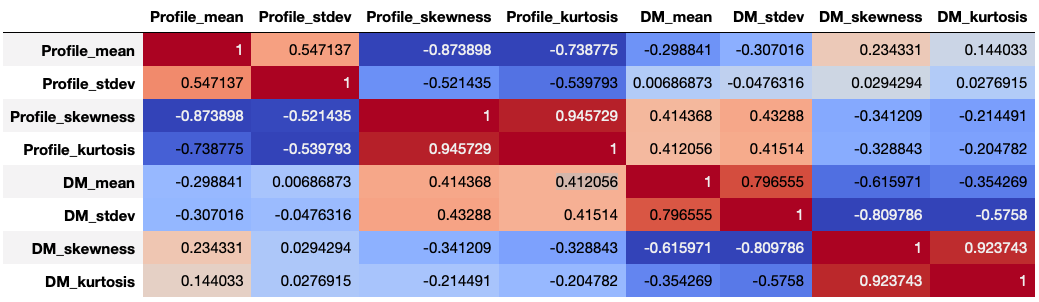
\includegraphics[width=1.0\textwidth]{CorrelationMatrix.png}
    \caption{Matriz de Correlaciones}
    \label{CorrMatrix}
\end{figure}

Puesto que algunos métodos se ven afectado por los \textit{features} irrelevantes, o por correlaciones elevadas entre ellos \cite{Kotsiantis14}, se ha decidido comparar la calidad de los modelos entrenados con el \textit{data set} completo y con un subconjunto de este sin variables correlacionadas, pudiendo asi determinar el conjunto de \textit{features} adecuados para cada modelo.\vspace{5mm}

Para la selección de \textit{features} no correlacionados, se ha procedido eliminando uno de dos correlacionados si y solo si estos presentan una correlación superior a 0.9.

\subsection{Visualization}

Como contamos con un dataset de 8 \textit{features}, para poderlo visualizar realizamos \textit{Principal Component Analysis}, proyectando los datos en un espacio de 2 dimensiones.

\begin{figure}[H]
    \centering
    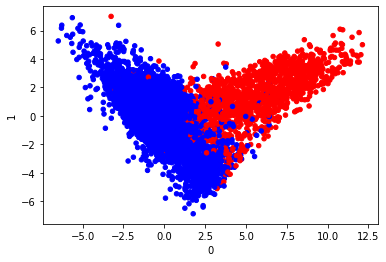
\includegraphics[width=0.7\textwidth]{PCAScatter.png}
    \caption{Scatter plot del PCA (2-dimensiones)}
    \label{ScatterPCA}
\end{figure}

Como se puede observar en la Figura \ref{ScatterPCA} existen a simple vista 2 grupos de datos (azul para los no púlsares y rojo para los púlsares). Se puede apreciar a demás que la franja entre ambos grupos parece ser clara, pudiendose dibujar una linea entre ambas clases, aunque existe una clara mezcla entorno a la linea de división. Se puede observar también como algunos puntos de ambas clases directamente escapan del conglomerado al que pertenecen.

\subsection{Clustering}

Por lo mencionado sobre en la Figura \ref{ScatterPCA} del apartado anterior, cabría esperar la existencia de 2 clusters.\vspace{5mm}

Scikit-learn proporciona diferentes métodos de clustering. Se ha decidido emplear $k$-means ya que trabaja correctamente con un número elevado de muestras y con un número medio de clusters \cite{Scikit:Clustering}, además de ser un método de propósito general. Para medir la calidad del clustering se ha empleado el índice de Calinski-Harabasz (CH). \vspace{5mm}

Ejecutando 50 veces $k$-means para $k \in [2..12]$, realizando la media de las ejecuciones, se ha obtenido que la mejor $k$ par el conjunto de datos estandarizados es $k = 4$. \vspace{5mm}

Como $k$-means trabaja con la distancia euclidiana, y puesto que esta tiende a "inflarse" con dimensiones elevadas \cite{Scikit:Clustering}, realizamos el clustering sobre el conjunto de datos tras realizar PCA.\vspace{5mm}

\begin{figure}[H]
    \centering
    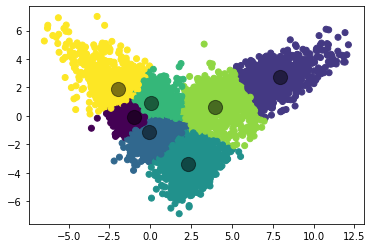
\includegraphics[width=0.8\textwidth]{ScatterKMeansPCA_7.png}
    \caption{Scatter plot del $k$-means de PCA}
    \label{ScatterKMeansPCA7}
\end{figure}

El valor óptimo obtenido es $k = 7$ (Figura \ref{ScatterKMeansPCA7}), con un sub-óbtimo destacado para $k = 4$. Esto nos permite darnos cuenta de la complejidad del problema, donde la variabilidd de los datos no púlsares es muy amplia, y aunque diferenciada de los púlsares, presenta subconjuntos. El conjunto de datos de púlsares parece ser más homojeneo, con dos subconjuntos en él.

%--------------------------------------
%  Resampling protocol
%--------------------------------------

\section{Resampling Protocol}\label{sec: resampling}

El protocolo de remuestreo empleado en todo momento en el trabajo ha sido \textit{10-Fold Cross Validation}. Este se ha aplicado en el entrenamiento de los diferentes métodos sobre un subconjunto de los datos, el \textit{training set}, del 80\% de los ejemplos, reservado el 20\% restantes para el \textit{test set}.\vspace{5mm}

Se ha decidido emplear $k = 10$ ya que al tener 17.898 ejemplos, aunque se haya empleado CV con el 80\% de los datos, queda jsutificado que son suficientes como para emplear dicha $k$.\vspace{5mm}

Excepcionalmente, no se ha utilizado este método para el modelo de Random Forests, ya que para optimizar los parámetros de este, se ha optado por utilizar como guía la medida \textit{Out of Bag} (OOB), ya que supone un coste computacional menor y la fiabilidad del resultado es prácticamente la misma. 

%--------------------------------------
%  Models
%--------------------------------------

\section{Modelos de Clasificación}

Los modelos de clasificación escogidos para el presente trabajo son: Nearest-neighbor, Logistic Regression, Lineas Support Vector Machines; en cuanto a modelos lineales, y Redes MLP y Random Forest, en cuanto a modelos no lineales.\vspace{5mm}

Se decidido estudiar la adecuación de estos modelos para el problema presentado de forma gradual, es decir, empleando desde modelo menos complejos a modelos más complejos, con tal de poder comparar tanto la adecuación de estos al problema, como la necesidad de emplear modelos más o menos complejos.\vspace{5mm}

Para la modelización se ha empleado únicamente la librería scikit-learn de Python. Como librerías de apoyo se han empleado Pandas, Numpy, Matplotlib, Seaborn, Pickle, StatsModels y Graphviz.

\subsection{Métodos Lineales}
\subsubsection{Nearest-neighbors}

Scikit-learn ofrece dos tipos de métodos nearest-neighbor supervisado:
\begin{itemize}
    \item \textbf{KNeighborsClassifier}: Algoritmo basado en el número $k$ de vecinos.
    \item \textbf{RadiusNeighborsClassifier}: Algoritmo basado en el número de vecinos dentro de un radio fijo de cada punto de entrenamiento.
\end{itemize}

Se ha decidido emplear el primero ya que es el algoritmo básico estandard de propósito general.\vspace{5mm}

Este método permite ajustar diferentes parámetros del modelo: el \textbf{algoritmo para el computo de los vecinos más cercanos} (BallTree, KDTree, Brute-force Search), el \textbf{tipo de métrica a emplear en las distancias} (Manhattan o Euclidea), y la \textbf{forma asignar pesos} (uniforme o inverso de la distancia).\vspace{5mm}

Empleando $GridSearchCV$, como se ha descrito en la Sección \ref{sec: resampling}, se ha buscado la mejor parametrización del modelo, empleando como posibles valores de vecinos el rango $[2,50]$.\vspace{5mm}

Entrenando con los parámetos descritos, y los datos estandarizados, se ha encontrado que el mejor modelo, con un error de training medio de 2.11\%, es el que cuenta la parametrización de la tabla \ref{BetterKNNParams}.

\begin{table}[H]
\centering
\begin{tabular}{|c|c|c|c|}
\hline
\textbf{$k$} & \textbf{Weights} & \textbf{Algoritmo} & \textbf{Métrica} \\ \hline
18 & distance & Ball Tree & Euclidea \\ \hline
\end{tabular}
\caption{Mejores parámetros obtenidos de KNeighborsClassifier}
\label{BetterKNNParams}
\end{table}

En test el error del mejor modelo encontrado tiene un ligero aumento hasta 2.21\%, lo cual se puede considerar muy aceptable dada la complejidad del problema y la sencillez de este primer modelo. \vspace{5mm}

Cabe destacar, como se podría esperar y se puede observar en la Tabla \ref{ConfMatrixKNN}, la clase Púlsar es la más perjudicada en predicciones, ya que es la que cuenta con menos ejemplos.

\begin{table}[H]
\centering
\begin{tabular}{|l|r|r|}
\hline
\textbf{\begin{tabular}[c]{@{}l@{}}Predicción\\ Real\end{tabular}} & \multicolumn{1}{l|}{\textbf{No púlsar}} & \multicolumn{1}{l|}{\textbf{Pulsar}} \\ \hline
\textbf{No púlsar} & 3230 & 19 \\ \hline
\textbf{Pulsar} & 60 & 271 \\ \hline
\end{tabular}
\caption{Matriz de confusión del mejor modelo KNN en test}
\label{ConfMatrixKNN}
\end{table}

Buscando el mejor modelo, pero con los \textit{features} seleccionados, es decir, sin los correlacionados, se ha obtenido el mismo hypertuning óptimo, pero con $k = 17$.\vspace{5mm}

Entrenando con los dato sin correlación se ha obtenido el mejor modelo con un error de training medio igual que con los datos correlacionados, pero un error de test muy ligeramente superior, 2.23\%.\vspace{5mm}

Ni el error de test en ambos, ni el tiempo de entrenamiento medio (0.092s con \textit{features} correlacionados y 0.081s sin correlacionados), son muy determinantes para decantarse por un conjunto de \textit{features} u otro.

\subsubsection{Logistic Regression}
Se ha decidido emplear regresión logística debido a que la salida que queremos predecir es binaria y resulta intuitivo utilizar esta técnica para dicho tipo de predicciones.\vspace{5mm}

La librería scikit-learn ofrece un método de regresión logísitca llamado LogisticRegression. Este permite introducir una serie de  parámetros que pueden ser ajustados. Para el presente trabajo, los parámetros que se han considerado más relevantes para estudiar son:\textbf{ la norma utilizada para la penalización (L1 o L2)}, $penalty$; \textbf{el parámetro de regularización inversa}, $C$; y \textbf{el algoritmo a utilizar en la optimización del modelo}, (\textit{liblinear} o \textit{saga}). \vspace{5mm}

Se ha empleado \textit{GridSearchCV} con valores posibles de C entre $1 \times 10^{-4}$ y $1 \times 10^{4}$ generados en una escala logaritmica.\vspace{5mm}

Entrenando el modelo con los parámetros indicados y utilizando los datos estandarizados, el mejor modelo que se ha encontrado con CV tiene como parámetros: penalty L1, el algoritmo $liblinear$ y el valor de $C = 4.28$. Curiosamente, para los datos sin \textit{features} correlacionados, los parámetros obtenidos resultan ser los mismos, lo que nos indica que la extracción de los \textit{features} es correcta ya que claramente no influyen en el modelo. \vspace{5mm}

El error de training medio obtenido en el CV utilizando los datos estandarizados con todos los \textit{features} es de 2.06\% y de 2.12\% para los datos sin los \textit{features} correlacionados.\vspace{5mm}

En el caso del error de testing, con el modelo obtenido indicando los parámetros optimizados, es de 2.23\% para los datos estandarizados. Para los datos sin \textit{features} correlacionados, en cambio, el error de testing sufre un ligero aumento hasta 2.56\%. \vspace{5mm}

Dada la reducción de complejidad del problema que supone la eliminación de las \textit{features}, el incremento del error en el segundo caso no supone un problema considerable. No obstante, debido a que el error es menor en el primer modelo y que el tiempo de ejecución de ambos resulta muy parecido, está justificada la decisión de quedarse con este antes que con el segundo. 

\subsubsection{Linear Support Vector Machine}
Se ha decidido emplear el kernel lineal en SVM ya que, dadas las conclusiones extraidas del análisis de los datos, estos parecen estar suficiente separados y tener una distribución adecuada para el kernel lineal, por la visualización en dos dimensiones.\vspace{5mm}

Scikit-learn, mediante el método LinearSVM permite hypertunear dos parámetros de especial relevancia: el \textbf{parámetro de regularización} $C$ y el \textbf{peso de las clases} (cada clase el mismo peso o balanceado).\vspace{5mm}

Empleando GridSearchCV, con posibles valores de $C\in[0.001, 0.01, 0.1, 1, 10, 100,\\ 1000]$, y acotando el número de iteraciones posibles de entrenamiento a 5.000; se ha encontrado que el mejor modelo es el que contempla $C = 1$ y el mismo peso en ambas clases.\vspace{5mm}

El error de training medio con dichos parámetros es 2.15\%, y el de test 2.37\%. Igual que con los modelos anteriores la precisión del modelo para no púlsar es mayor, 98\%, que la de púlsar, 93\%.\vspace{5mm}

Entrenando con los datos sin \textit{features} correlacionados se obtiene que el mejor modelo es con $C = 100$ y con el mismo peso en ambas clases. En este caso se presenta un mejor error en test, 2.29\%, consiguiendo un aumento en el \textit{recall} de la clase púlsar. De 80\% a 82\%, manteniendo el \textit{recall} de la clase no púlsar en 99\%.\vspace{5mm}

\subsection{Métodos no lineales}
\subsubsection{Redes MLP}

Para el desarrollo de redes MLP, scikit-learn ofrece suficiente potencia como para no ser necesario recurrir a otras librerías, por lo que emplearemos el método MLPClassigier de scikit.\vspace{5mm}

Este método ofrece varios parámetros a ajustar, de los cuales se trabajará únicamente con: \textbf{neuronas de las capas interiores}, \textbf{función de activación} y \textbf{$\alpha$}.\vspace{5mm}

Otro parámetros interesantes podrían ser el \textit{solver}. Se empleará el disponible por defecto, $adam$, ya que trabaja correctamente con \textit{datasets} relativamente grandes en cuanto a \textit{samples} como HTRU2 \cite{Scikit:MLPClassifier}.\vspace{5mm}

El resto de parámetros, como el learning rate o el momentum, o no estan disponibles para $adam$ o se han considerado no relaventes para el problema, puesto que este no presenta una complejidad suficientemente elevada como para necesitar, por ejemplo, el momentum para la aceleración de la optimización.\vspace{5mm}

Para lo parámetros si consideraros, se ha creado un grid con los siguientes elementos:
\begin{itemize}
    \item $hidden\_layer\_sizes \in [(20,), (40,), (50,), (70,), (100,), (20,20,20), \\(50,50,50), (20,50,200), (50,100,50)]$
    \item $activation \in [logistic, tanh, relu]$
    \item $\alpha \in [1.e-01, 1.e-02, 1.e-03, 1.e-04, 1.e-05, 1.e-06]$
\end{itemize}

Realizando esta seleccion de parámetros se ha intentado cubrir una amplia gama de posibilidades, especialmente con $hidden\_layer\_sizes$, de acuerdo a la complejidad del problema (8 \textit{features}).\vspace{5mm}

Realizando CV sobre el set con \textit{featrues} correlacionados y sin, se ha encontrado que las mejores redes posibles son las siguientes:
\begin{table}[H]
\centering
\begin{tabular}{l|c|c|c|}
\cline{2-4}
 & \textbf{Capas Ocultas} & \textbf{Función de Activación} & \textbf{$\alpha$} \\ \hline
\multicolumn{1}{|l|}{\textbf{Corr}} & (50,100,50) & tanh & 0.1 \\ \hline
\multicolumn{1}{|l|}{\textbf{No corr}} & (20,20,20) & logistic & 0.01 \\ \hline
\end{tabular}
\caption{Mejores parametros para MLPClasssifier (encontrados con CV)}
\label{GridSearchMLPResults}
\end{table}

Se puede apreciar en la Tabla \ref{GridSearchMLPResults} como la eliminación de los \textit{features} correlacionados lleva a la obtención de un modelo más simplificado, reduciendose el número de neuronas por capa. En cuanto a la función de activación es remarcable como para ambos conjuntos de datos funciona mejor una función de tipo curva, que no una función de tipo recta como ReLU.\vspace{5mm}

El modelo entrenado con el set de datos normal estandarizado ha presentado un error de entrenamiento medio de 1.89\% y un error de test superior, de 2.32\%. Mientras que para el modelo entrenado con datos sin \textit{features} correlacionados el error medio de entrenamiento ha sido de 1.89\% y el de test de 2.23\%.\vspace{5mm}

Aunque el error de test en ambos modelos se encuentra en la linea de los modelos lineales, MLP permite conseguir una mayor precisión, y se adapta mejor a la falta de ejemplos de púlsares como se puede observar en la Tabla \ref{ConfMatrixMLP}, aunque empeora en la detección de no púlsares.

\begin{table}[H]
\centering
\begin{tabular}{|l|r|r|}
\hline
\textbf{\begin{tabular}[c]{@{}l@{}}Predicción\\ Real\end{tabular}} & \multicolumn{1}{c|}{\textbf{No púlsar}} & \multicolumn{1}{c|}{\textbf{Púlsar}} \\ \hline
\textbf{No púlsar}                                                 & 3218                                    & 31                                   \\ \hline
\textbf{Púlsar}                                                    & 52                                      & 279                                  \\ \hline
\end{tabular}
\caption{Matriz de confusión del mejor modelo MLP (Corr) en test}
\label{ConfMatrixMLP}
\end{table}



\subsubsection{Random Forest}
Se ha decidido emplear este modelo ya que en Random Forests no es necesario estandarizar los datos, y además funciona bien en problemas de clasificación cuyos datos de diferentes clases estan desequilibrados, que es lo que ocurre en el problema que nos ocupa. \vspace{5mm}

Los métodos de scikit-learn utilizados son dos. El método para el propio modelo, \textit{RandomForestClassifier} y \textit{compute\_class\_weight}, que permite calcular el mejor peso para las diferentes clases del problema. Estos pesos sirven para compensar el desequilibrio de datos que pueda haber entre diferentes clases.\vspace{5mm}

El principal parámetro que admite \textit{RandomForestClassifier} es \textit{n\_estimators}, que se corresponde con el número de \textit{decision trees} que debe generar el Random Forest. Para este parámetro se ha decidido probado valores que van entre 10 y 1000, un rango considerablemente amplio. Posteriormente se ha probado entre 100 y 250, al observar primeramente que es entre esos valores donde la variabilidad del resultado cobraba importancia. \vspace{5mm}

Como ha sido explicado en la Sección 4, para este modelo, utilizaremos la puntuación del propio modelo, conocida como OOB. Ésta permite hypertunear el parámetro de número de árboles y así saber cuál es el valor de este parámetro que da un mejor resultado. \vspace{5mm}

Para el caso de los datos normales (sin estandarizar y con todos los \textit{features}), el número de árboles que mejor puntuación ha obtenido es 120, con una puntuación OOB de 0.019 y un error de training casi ínfimo, de 0.007. Al predecir los correspondientes datos de test con este modelo, el error de test resulta ser 2.37\%.

\begin{table}[H]
\centering
\begin{tabular}{|l|r|r|}
\hline
\textbf{\begin{tabular}[c]{@{}l@{}}Predicción\\ Real\end{tabular}} & \multicolumn{1}{l|}{\textbf{No púlsar}} & \multicolumn{1}{l|}{\textbf{Pulsar}} \\ \hline
\textbf{No púlsar} & 3210 & 29 \\ \hline
\textbf{Pulsar} & 60 & 271 \\ \hline
\end{tabular}
\caption{Matriz de confusión del mejor modelo de RF en test}
\label{ConfMatrixRF}
\end{table}

En cambio, para el caso de los datos sin \textit{features} correlacionados, el número óptimo de arboles de decisión ha sido 100. La puntuación OOB en este caso ha sido 0.019 y el error de training ha sido 0.007, otra vez. En este caso, no obstante, el error de test ha sido de 2.56\%, un poco peor que el resultado anterior.\vspace{5mm}

De la misma forma que ocurría con el modelo MLP, Random Forest se mantiene en la línea de los modelos lineales en cuanto a los errores de test, no obstante también empeora en la identificación de pulsares. \vspace{5mm}

%--------------------------------------
%  Final Model
%--------------------------------------

\section{Modelo final}

\begin{table}[H]
\centering
\begin{tabular}{lcccc}
\hline
\multicolumn{1}{c}{Método} & Accuracy & Recall & Precision & F-Score \\ \hline
$k$-NN (Corr) & \textbf{0.98} & 0.91 & \textbf{0.96} & \textbf{0.93} \\
$k$-NN (No corr) & \textbf{0.98} & 0.90 & \textbf{0.96} & \textbf{0.93} \\
Logistic Regression (Corr) & \textbf{0.98} & 0.91 & \textbf{0.96} & \textbf{0.93} \\
Logistic Regression (No corr) & 0.97 & 0.88 & \textbf{0.96} & 0.92 \\
Linear SVM (Corr) & \textbf{0.98} & 0.90 & \textbf{0.96} & 0.92 \\
Linear SVM (No corr) & \textbf{0.98} & 0.90 & 0.95 & \textbf{0.93} \\
MLP (Corr) & \textbf{0.98} & \textbf{0.92} & 0.94 & \textbf{0.93} \\
MLP (No corr) & \textbf{0.98} & 0.91 & 0.95 & \textbf{0.93} \\
Random Forest (Corr) & \textbf{0.98} & 0.91 & 0.95 & \textbf{0.93} \\
Random Forest (No corr) & \textbf{0.98} & 0.91 & 0.94 & \textbf{0.93} \\ \hline
\end{tabular}
\caption{Accuracy, Recall, Precision y F-Score obtenidos con cada conjunto de datos y método}
\label{TotalCompareTable}
\end{table}

Con tal de escoger un método final, se ha confeccionado la Tabla \ref{TotalCompareTable} para así poder comparar los diferentes resultados de Accuracy, Recall, Precision y F-Score para los distintos métodos y conjuntos de datos utilizados. \vspace{5mm}

Al comparar estos resultados, se observa que todos los métodos obtienen resultados muy parecidos, lo que dificulta la elección de un método en concreto. Es por ello que también es necesario estudiar en profundidad los resultados para ambas clases de forma más concreta. Con este motivo se ha generado la Tabla \ref{RecallPrecisionCompareTable}. \vspace{5mm}

Como se ha comentado en secciones anteriores, se observa una clara diferencia entre los modelos lineales y no lineales en cuanto al resultado que los segundos dan sobre la predicción de púlsares, la cual es claramente peor en términos de precisión. Sin embargo, para la predicción de no púlsares, los resultados son prácticamente iguales en todos los modelos. \vspace{5mm}

También se observa que, en los casos en los que se utiliza el conjunto de datos sin \textit{features} correlacionados, para la detección de púlsares, la precisión sube a costa del recall. Es por esto que es preciso rechazar los métodos en los que se utilizan datos sin \textit{features} correlacionados. Siendo de especial interes también la reducción en cuanto a complejidad que aportan.\vspace{5mm}

Finalmente, es intuible la selección de un método lineal. Por una parte, como se ha comentado, estos dan un mejor resultado para la predicción de púlsares y por otra, claramente su sencilleza ante los métodos no lineales hace que estos tengan un coste computacional mucho menor, interesante para aplicaciones en tiempo real, por ejemplo. Entre estos, se observa que k-NN y Logistic Regression tienen un comportamiento casi idéntico. Debido a la simplicidad algorítmica del primero y a la facilidad para entender lo que realmente está ocurriendo al ejecutarse, hemos decidido quedarnos con k-NN como mejor modelo, aunque hacemos incisión en el hecho de que Logistic Regression también es un método a tener en cuenta.
\begin{table}[H]
\centering
\begin{tabular}{lcccc}
\hline
\multicolumn{1}{c}{\multirow{2}{*}{Método}} & \multicolumn{2}{c}{Recall} & \multicolumn{2}{c}{Precision} \\ \cline{2-5} 
\multicolumn{1}{c}{} & No púlsar & Púlsar & No púlsar & Púlsar \\ \hline
$k$-NN (Corr) & 0.99 & 0.82 & 0.98 & 0.93 \\
$k$-NN (No corr) & 0.99 & 0.81 & 0.98 & 0.94 \\
Logistic Regression (Corr) & 0.99 & 0.82 & 0.98 & 0.93 \\
Logistic Regression (No corr) & \textbf{1.00} & 0.77 & 0.98 & \textbf{0.95} \\
Linear SVM (Corr) & 0.99 & 0.80 & 0.98 & 0.93 \\
Linear SVM (No corr) & 0.99 & 0.82 & 0.98 & 0.93 \\
MLP (Corr) & 0.99 & \textbf{0.84} & 0.98 & 0.90 \\
MLP (No corr) & 0.99 & \textbf{0.84} & 0.98 & 0.91 \\
Random Forest (Corr) & 0.99 & \textbf{0.84} & 0.98 & 0.91 \\
Random Forest (No corr) & 0.99 & \textbf{0.84} & 0.98 & 0.90 \\ \hline
\end{tabular}
\caption{Recall y Precision para cada clase obtenidos con cada conjunto de datos y método}
\label{RecallPrecisionCompareTable}
\end{table}

%--------------------------------------
%  Conclusions
%--------------------------------------

\section{Conclusiones}

\subsection{Autoevaluación}
El desarrollo de todo el conjunto del trabajo se ha realizado de forma pautada y premeditada, hecho que ha permitido un correcto desarrollo de este, pudiendose cumplir todos los objetivos prefijados al inicio.\vspace{5mm}

Hemos podido analizar de forma adecuada los datos, pudiendo llegar a asegurar que existe una clara relación entre las variables de entrada dadas por el problema y la clasificación de estos datos en Púlsares o no Púlsares. Esta afirmación está justificada debido a que en todos los métodos de aprendizaje automatico que se han utilizado la predicción que se ha dado de los datos ha sido suficientemente fiable.\vspace{5mm}

También hemos podido probar una gama amplia de posibilidades por cada uno de los modelos estudiados gracias a la librería scikit-learn, pudiendo así tratar de conseguir mejores modelos.

\subsection{Conclusiones personales y científicas}
Desde un punto de vista personal, consideramos que tener la posibilidad de estudiar un conjunto de datos como el estudiado nos ha permitido entender de una forma más profunda como funcionan los diferentes modelos de aprendizaje supervisado, como tratar con grandes cantidades de datos y como interpretar los diferentes resultados. Además, aplicando las tecnicas empleadas a un conjunto de datos real, se ha dado un sentido y aplicación real a dichos métodos, pudiendose profundizar más en ellos.\vspace{5mm}

En el plano cientifico, queremos destacar la viabilidad de emplear los modelos desarrollados  para este problema. Dada la precisión que estos presentan, no sería descabellado emplearlos en nuevos datos obtenidos sobre otras estrellas diferentes. Así, aquellos físicos que esten estudiando y recopilando datos sobre estrellas puedan utilizar estos modelos de predicción para enfocar y realizar sus estudios de forma más eficiente.

\subsection{Posibles extensiones y limitaciones}
La principal limitación del problema ha sido el desequilibrio que existe entre las clases dadas, ya que el número de ejemplares no-púlsares es mucho mayor que el de púlsares. Esto ha hecho que en los métodos utilizados la precisión de predicción de púlsares fuera mucho más limitada que la de no-púlsares. Aun asi se ha decidido no emplear tecnicas para mejorar el desequilibrio, puesto que los resultados obtenidos son de especial relevancia, aunque sería interesante contemplar la posibilidad de intentar mejorar el balanceo de clases para tratar de encontrar una mejora en la predicción. \vspace{5mm}

Otra posible extensión de este problema sería probar otros modelos de aprendizaje supervisado sobre los datos y compararlos con los ya estudiados para observar posibles diferencias y/o mejoras. Algunos de estos modelos podría ser versiones mejoradas o más rapidas de los aqui estudiados, para poderlos emplear en experimentos en tiempo real. 

\newpage

%--------------------------------------
%  Bibliography
%--------------------------------------

\nocite{*}
\printbibliography

\end{document}
